
\chapter{面向交通资产属性识别的长尾数据构建与增强验证}

\section{引言}

在完成交通资产目标检测之后，还需要进一步对目标对应的局部区域进行属性识别，以判断其几何形态、工作状态及潜在异常类型。与仅输出目标类别的检测任务相比，属性识别更关注目标的细粒度语义描述，要求系统不仅回答“该资产是什么”，还要回答“该资产处于什么状态、是否存在异常以及异常表现为何种具体形式”。本章关注的重点在于“如何将行业规范、运维经验和视觉先验转化为面向特定异常类型的生成控制信号，并以此定向改善属性识别所依赖的训练分布”。在这一意义上，知识不再作为识别后的附加解释，而是被前置为长尾数据生成与训练集构建中的驱动因素。

针对上述问题，本文面向交通资产属性识别任务，提出一种领域知识引导长尾数据生成与增强方法。该方法以真实采集样本为基础，以交通领域知识为约束，通过生图模型定向补充难以采集的异常长尾样本，进而增强属性识别训练数据中关键异常字段的覆盖度。

本章主要介绍交通资产属性识别任务下的总体技术路线、任务定义、数据构建方式、知识到生成约束的映射机制，以及基于 Qwen3-VL-4B-Instruct 的属性识别模型训练方案。其核心目标不是单独追求“异常生成”本身，而是围绕属性识别需求，通过领域知识引导塑造训练分布，提升交通资产属性识别模型在关键长尾异常字段上的识别准确率，同时保持整体属性识别能力。

\section{领域知识引导长尾数据生成的总体技术路线}

图~\ref{fig:problem_definition_pipeline} 给出了“交通资产属性识别任务定义与领域知识引导长尾数据生成总体流程图”。该流程并非单一的图像生成或模型微调步骤，而是围绕“任务定义—知识约束—样本构建—模型训练—效果验证”形成的完整技术闭环。具体而言，整体流程可以概括为以下五个环节：

\begin{enumerate}
    \item \textbf{任务定义与属性体系构建}：首先基于交通资产巡检需求，将信号灯、路灯、交通标志牌、井盖、垃圾桶等对象的识别目标细化为结构化属性集合，明确哪些属性属于常规上下文属性，哪些属性属于异常风险属性。
    \item \textbf{领域知识抽取与约束表达}：从国家标准、材料规范、运维经验和真实视觉先验中提取可转化为 Prompt 约束的知识规则，用于限定异常类型、异常等级、异常位置以及背景保持方式。
    \item \textbf{知识引导生成与批量构造}：基于参考图像执行局部异常编辑，通过 Prompt 迭代优化与多生成模型对比确定主生成模型，并据此批量构造面向关键异常属性的长尾补充样本集。
    \item \textbf{训练集组织与监督微调}：将真实采集样本与通过质量控制的生成异常样本按统一格式组织为多模态指令数据，分别构造仅真实样本训练集和长尾增强训练集，并在一致训练范式下训练同构识别模型。
    \item \textbf{统一评测与结果分析}：在统一测试集上，从样本级严格准确率、属性级准确率、异常属性准确率以及正常--异常性能差距等角度评估模型，并进一步分析关键异常字段及商用大模型基线表现。
\end{enumerate}

上述流程的关键点在于：领域知识并非作为后验解释性信息附加在模型输出之后，而是被前置为训练数据构建过程中的显式控制信号。由此，图~\ref{fig:problem_definition_pipeline} 所示流程实际上实现了从“规范知识”到“可训练样本”，再到“交通资产属性识别模型”的系统性映射。

\begin{figure}[htbp]
    \centering
    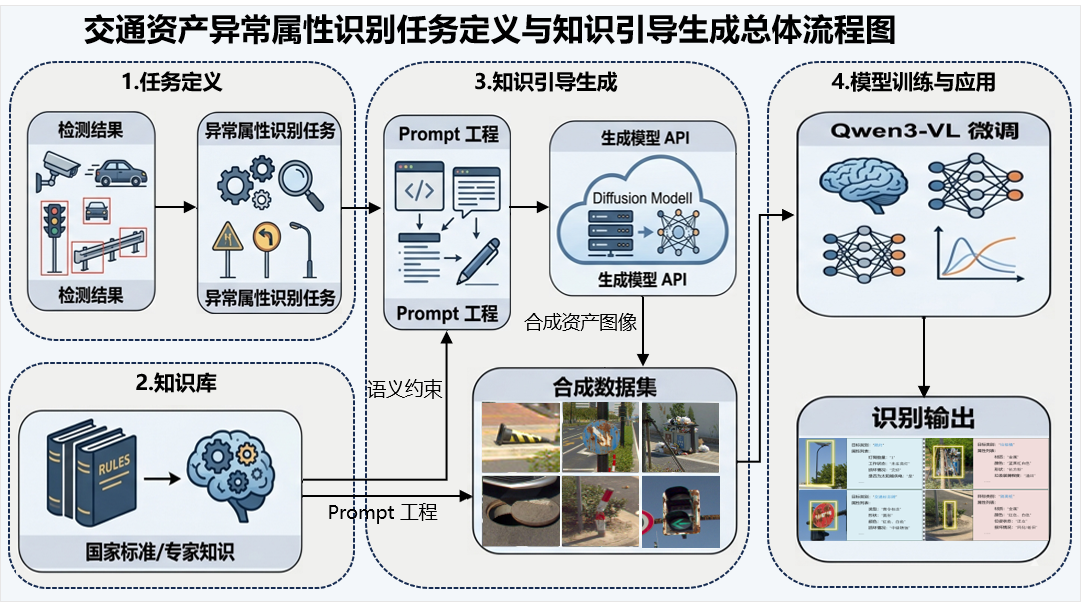
\includegraphics[width=1.0\textwidth]{logo/交通资产异常属性识别任务定义与知识引导生成总体流程图.png}
    \caption{交通资产属性识别任务定义与领域知识引导长尾数据生成总体流程图}
    \label{fig:problem_definition_pipeline}
\end{figure}

\section{面向属性识别增强的问题定义与研究动机}

设目标检测阶段输出的交通资产候选区域集合为
\[
\mathcal{B}=\{b_1,b_2,\ldots,b_N\},
\]
其中 $b_i$ 表示第 $i$ 个候选目标对应的局部裁剪图像。对于每个候选区域，本文并不将其建模为单一分类问题，而是输出结构化属性集合：
\[
 y_i = \{(a_{i,j}, v_{i,j})\}_{j=1}^{m_i},
\]
其中 $a_{i,j}$ 表示第 $j$ 个属性键，$v_{i,j}$ 表示对应属性值，$m_i$ 为该目标可见属性的数量。不同目标的属性集合并不完全相同，例如信号灯包含“类型”“工作状态”“颜色”“破损情况”“设备类型”等字段，井盖则包含“形状”“隐患情况”与“表面图案”等字段。

因此，本文所研究的交通资产属性识别任务可视为条件结构化预测问题。给定图像区域 $x_i$ 与任务提示模板 $t_i$，模型学习映射函数
\[
 f_{\theta}:(x_i,t_i)\rightarrow y_i,
\]
并输出可解析的 JSON 结构。该建模方式既保留了属性间的语义依赖关系，也便于后续按属性粒度开展评测与分析。

交通资产异常样本稀缺并非偶然现象，而是由设施运维机制、采集方式和标注成本共同造成的。首先，城市道路设施在大部分时间内处于正常可用状态，严重异常样本本身出现频率较低；其次，异常状态具有突发性和离散性，依赖大规模外业巡检也难以在有限时间内覆盖所有异常形态；再次，异常属性往往依赖一定的工程知识，例如锈蚀等级、移位程度或结构变形方向并不是普通视觉标签，而是与设施材料、受力模式及运维标准密切相关的专业概念。

真实属性识别样本来源于第二章介绍的 WHU-Infra3D 数据集。本文以数据集中的二维标注框为基础，先计算每个标注框对应目标与当前全景拍摄曝光点之间的距离，仅保留距离曝光点 20\,m 范围内的目标；随后将保留标注框按 1.5 倍比例外扩，裁剪得到面向属性识别的局部图像。该流程既保证了目标在全景图中的可辨识性，也为后续异常编辑提供了统一的参考视图。

经过上述筛选后，真实样本中常规状态占据绝对多数，而异常状态在多个关键字段上明显缺失，主要表现为：1）“损坏情况”几乎被“完好”主导，弯曲、结构损坏和严重损坏等状态极为稀缺；2）“老化情况”中与锈蚀和风化老旧相关的异常等级样本极少；3）“隐患情况”缺少“微微移位”“移开一半”和“完全移开”等关键高风险类别；4）“垃圾是否装满”仅包含“否”，未覆盖“满至边缘”与“溢出”等运维场景中更具管理价值的状态。

若直接在上述数据上训练模型，模型在优化过程中会优先适配高频正常值，从而导致总体准确率可能看似较高，但在真正关键的低频异常类别上表现不稳定。这意味着，仅凭真实采集数据难以支撑可靠的交通资产属性识别系统，尤其难以稳定覆盖关键异常字段。

为缓解真实训练数据中的长尾问题，本文引入基于领域知识引导的异常样本补充策略。其基本思想是：保留真实采集样本所提供的道路场景真实性与常规分布，再利用知识引导的图像生成方法定向补足原训练集中稀缺的异常属性值，从而构造对照明确的训练集组织方式。记
\[
D_{\mathrm{real}}^{\mathrm{tr}}
\]
为仅包含真实采集样本的训练集，
\[
D_{\mathrm{gen}}^{\mathrm{aug}}
\]
为基于领域知识引导生成的长尾补充样本集，则长尾增强训练集可表示为
\[
D_{\mathrm{aug}}^{\mathrm{tr}} = D_{\mathrm{real}}^{\mathrm{tr}} \cup D_{\mathrm{gen}}^{\mathrm{aug}}.
\]

在此基础上，后续实验分别基于 $D_{\mathrm{real}}^{\mathrm{tr}}$ 与 $D_{\mathrm{aug}}^{\mathrm{tr}}$ 构造同构属性识别器，并在统一测试集上比较两者表现，以分析生成长尾数据对整体属性识别能力、关键异常字段识别能力以及常规属性保持能力的影响。该研究思路的核心目标不是以生成数据替代真实数据，而是将其作为对真实训练分布的定向补充。

\section{领域知识引导的长尾异常样本构建}

本文将用于异常样本生成的知识来源概括为三类：
\begin{enumerate}
    \item \textbf{规范知识}：来自交通设施设计、维护和外观要求相关的国家标准与行业规范，用于约束颜色、材质、结构形式以及设施的合理外观边界。例如，《道路交通标志和标线 第2部分：道路交通标志》（GB 5768.2—2022）可用于约束交通标志牌的颜色配置、版面结构与设置逻辑，《道路交通反光膜》（GB/T 18833—2012）可用于约束反光材料的等级特征与视觉表现 \cite{gb5768_2022, gbt18833_2012}；
    \item \textbf{运维经验知识}：来自交通设施巡检和养护场景中的经验总结，用于描述不同异常通常出现的位置、形成机理以及严重程度差异；
    \item \textbf{视觉先验知识}：来自真实样本观察，用于总结锈蚀纹理、弯折方向、破损边缘、移位尺度、满溢堆积方式等具体视觉表现。
\end{enumerate}

在此基础上，本文围绕交通信号灯、路灯、交通标志牌、隔离桩、井盖、垃圾桶等对象，整理出对应的结构化属性体系。该属性体系既包含“类型”“颜色”“材质”“工作状态”等上下文属性，也包含“损坏情况”“破损情况”“老化情况”“隐患情况”“垃圾是否装满”等异常相关属性。前者用于提供对象语义与外观上下文，后者则直接服务于异常识别目标。

为使领域知识能够被生图模型有效利用，本文将其转化为面向局部编辑任务的生成约束。对于给定参考图像 $x_{ref}$，设其知识描述为
\[
 k=(o, a^{\mathrm{ctx}}, a^{\mathrm{abn}}, r, c),
\]
其中 $o$ 表示对象类型，$a^{\mathrm{ctx}}$ 表示需要保持稳定的上下文属性集合，$a^{\mathrm{abn}}$ 表示目标异常属性，$r$ 表示允许编辑的空间区域，$c$ 表示一致性约束，包括背景保持、光照连续、局部几何合理与非目标区域不改动等要求。生成模型接收参考图像与文本 Prompt 后，仅在受控区域内引入指定异常状态，从而得到异常图像 $\tilde{x}$：
\[
\tilde{x} = \mathcal{G}(x_{ref}, k, p).
\]

其中 Prompt $p$ 不再只是笼统描述“生成一个损坏目标”，而需要明确对象类型、异常位置、异常等级以及必须保持不变的内容。例如，对于“中级锈蚀交通标志牌”，Prompt 会强调锈蚀应主要集中于金属支撑件和边缘区域，表面反光膜不应被整体重绘，背景道路与周围设施保持不变。通过这种方式，生成样本不仅具有目标异常语义，还能够尽可能保持与真实道路场景一致的局部纹理和上下文结构。

在上述知识映射机制的基础上，本文进一步总结了适用于交通资产异常生成任务的 Prompt 工程设计原则。这些原则并非仅服务于“生成一张看起来合理的图片”，而是直接面向后续识别模型训练的数据可用性。总体而言，本文主要遵循以下四项原则：

\begin{enumerate}
    \item \textbf{单目标约束原则}：每条 Prompt 尽量只针对单一交通资产对象进行编辑，避免生成模型在多目标场景中发生注意力漂移，从而造成异常位置错配或对象主体改变；
    \item \textbf{局部编辑优先原则}：优先采用“参考图像 + 局部异常编辑”的生成方式，而非重新生成整幅场景图像，以最大程度保持真实道路背景、光照关系和上下文结构；
    \item \textbf{细节显式化原则}：对于锈蚀、弯折、凹陷、破裂、满溢等异常状态，不使用过于抽象的描述，而是显式给出异常部位、异常强度和可见视觉细节，以减小模型对异常语义的自由发挥空间；
    \item \textbf{环境锁定原则}：在 Prompt 中明确强调道路背景、其他交通设施、非目标区域和整体视角保持不变，防止生成模型在目标外区域引入额外变化，从而污染训练数据分布。
\end{enumerate}

上述原则共同作用的结果，是使生成数据不仅在视觉上“像异常”，更在训练意义上“可作为异常识别样本使用”。

在实际实验中，高质量 Prompt 往往并非一次设计即可得到，而需要通过多轮生成—观察—修订的方式逐步优化。为此，本文采用迭代式 Prompt 优化策略，其更新过程可表示为
\[
p^{(t+1)} = \Psi(p^{(t)}, r^{(t)}),
\]
其中 $p^{(t)}$ 表示第 $t$ 轮 Prompt，$r^{(t)}$ 表示对当前生成结果的误差观察与问题归纳，$\Psi$ 表示基于反馈信息对 Prompt 进行修订的更新函数。

在该过程中，研究者首先对生成样本进行人工观察与规则分析，重点检查以下问题：异常程度是否足够清晰、异常位置是否与预期一致、背景是否被错误修改、形变是否符合材料特性与受力逻辑、以及生成结果是否支持后续结构化属性标注。若发现问题，则通过补充异常细节、强化空间约束、限定材料特征或增加保真约束等方式对 Prompt 进行修订。经过多轮迭代后，Prompt 会逐渐从粗略描述演化为具有较强约束性的生成指令，从而显著提升异常样本的稳定性与工程可用性。

\begin{figure}[htbp]
    \centering
    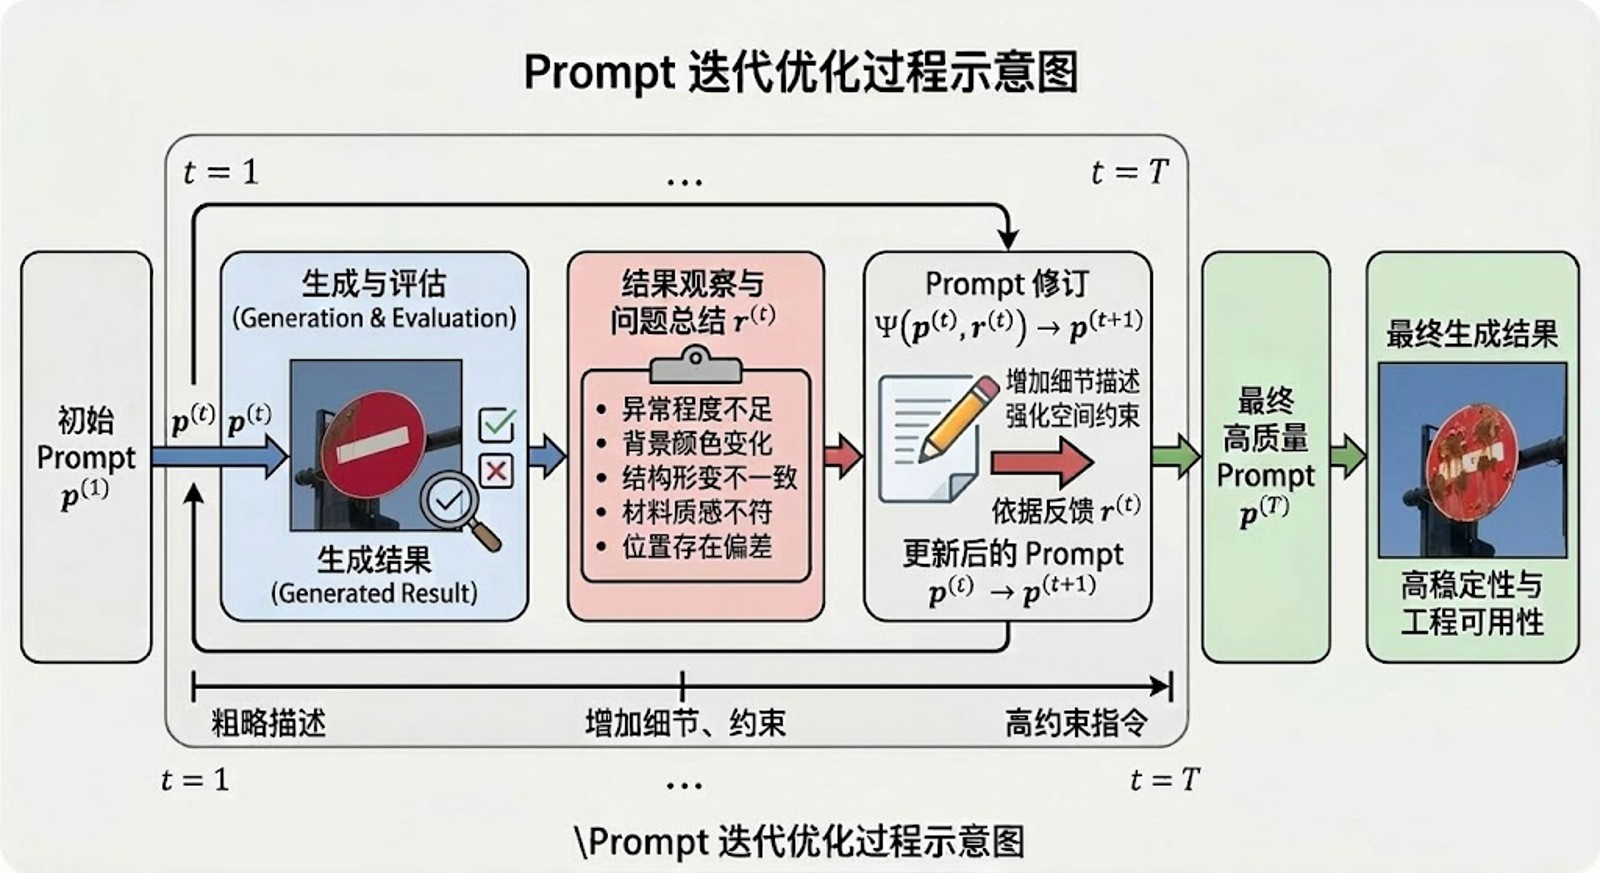
\includegraphics[width=1.0\textwidth]{logo/prompt迭代优化过程示意图.jpg}
    \caption{Prompt 迭代优化过程示意图}
    \label{fig:prompt_iteration}
\end{figure}

\section{生成模型选择策略}

为了使生成数据真正服务于交通资产属性识别增强，本文并不预设某一生成模型天然适合本任务，而是首先将“生成模型选择”视为一个面向工程可用性的比较问题。其核心不在于比较候选模型生成图像的视觉冲击力，而在于判断它们能否稳定完成受领域知识约束的局部异常编辑任务，即在保持目标主体、道路背景与上下文结构基本稳定的前提下，准确注入指定异常属性。换言之，本文关注的不是“谁更会作图”，而是“谁更适合被纳入交通资产异常样本批量构造流程”。

这一选择策略与前文提出的领域知识引导生成路线是紧密衔接的。在第四章前半部分，本文已经完成了异常类型定义、属性值设计、Prompt 模板约束以及局部编辑目标的形式化描述，因此生成模型在本章中的角色并不是自由创作，而是执行一种“受约束的异常编辑”任务：给定真实参考图像、对象类别、异常部位、异常等级和背景保持要求，模型需要输出一张既符合异常语义、又尽量保留原始场景结构的信息增强样本。如果候选模型无法稳定满足这些约束，那么即便其视觉效果较强，也难以真正用于后续结构化属性标注与识别训练。

基于这一认识，本文将生成模型选择过程划分为三个层次。第一层是\textbf{可编辑性筛查}，即判断模型是否能够围绕指定交通资产对象执行局部异常注入，而不是对整幅图像进行大幅重绘；第二层是\textbf{数据可用性比较}，即在统一参考图像、统一 Prompt 模板和统一异常属性约束下，比较不同模型在结构保持、异常表达和背景稳定性方面的综合表现；第三层是\textbf{批量构造适配性判断}，即进一步评估该模型是否适合作为统一主模型服务于后续大规模数据生成，包括输出风格是否稳定、异常等级是否可控、是否便于形成一致的训练分布。通过这样的分层筛选，本文希望确保最终选出的主生成模型不仅“单张效果较好”，而且“批量使用时仍然可靠”。

在具体评价准则上，本文构建了五维评价框架，用以统一比较候选模型在交通资产异常编辑任务中的表现。评价维度包括结构一致性、异常真实性、局部可控性、背景稳定性以及工程可用性，分别对应“目标是否仍是原对象”“异常是否足够可信”“异常是否出现在预期区域”“非目标区域是否保持稳定”以及“生成结果是否支持后续结构化属性标注”。其中，前四个维度主要衡量单张样本质量，第五个维度则更强调样本进入训练流水线后的实际价值。也就是说，本文最终选择主生成模型的标准，并不是某一单一指标最高，而是要求模型在多维约束下具有更强的整体均衡性。

此外，本文并未采用“多个生成模型混合使用”的策略，而是优先选择一个性能更稳定的统一主模型。这一决策主要出于两点考虑：其一，多模型混合虽然可能在视觉风格上带来更多样性，但也容易引入额外的分布不一致性，增加后续属性识别训练中的噪声来源；其二，统一主模型更有利于控制异常等级、背景扰动和局部编辑方式的一致性，从而使长尾补样过程更接近“按知识模板定向扩充训练分布”，而不是“随机增加若干视觉变体”。因此，在完成候选模型比较之后，本文将选择综合表现最优且稳定性最强的模型，作为后续异常样本批量构造的唯一主生成器。

在主生成模型确定之后，本文不再额外设计逐样本筛选流程，而是直接基于统一的属性模板、参考图像和 Prompt 约束，批量构造面向关键异常状态的长尾补充样本。该批量构造过程保持对象类别、异常类型、异常等级和局部编辑区域的一致约束，使生成结果能够按预设属性空间成规模补充训练数据。

\section{长尾数据增强的交通资产属性识别}

在完成长尾异常样本构建之后，本文进一步关注一个核心问题：这些面向异常属性补充得到的训练样本，能否真正转化为交通资产属性识别模型的判别能力。为此，本节不再将属性识别视为若干彼此独立的字段分类任务，而是将其统一建模为\textbf{“图像条件下的结构化属性生成”}问题：给定交通资产图像 $I$ 以及属性定义集合 $\mathcal{A}=\{a_1,a_2,\dots,a_K\}$，模型需要输出对应的属性结果
\[
Y=\{y_1,y_2,\dots,y_K\}, \qquad y_k \in \mathcal{V}(a_k),
\]
其中 $\mathcal{V}(a_k)$ 表示属性 $a_k$ 的合法取值空间。该建模方式使模型不仅要识别局部视觉线索，还要同时满足属性语义约束、字段间一致性约束以及结构化输出约束。

基于上述认识，本文采用多模态指令模型作为属性识别器。其原因在于，交通资产属性识别并不只是“看图分类”，还要求模型能够理解属性字段的含义、区分正常状态与异常状态的细粒度差异，并以统一格式输出多字段结果。相比为每个属性单独训练一个分类头，统一的结构化生成范式更适合承载“类别识别—异常判断—结果组织”这一完整推理链条，也更符合后续工程部署中一次输入、一次输出完整属性结果的应用需求。

因此，本文将每个训练样本组织为“图像 + 属性说明 + 结构化答案”的监督样式，其中图像提供视觉证据，属性说明明确任务边界与字段语义，结构化答案则给出标准属性标注。模型学习的目标可以表示为条件生成
\[
p_{\theta}(Y \mid I, \mathcal{A}),
\]
即在给定交通资产图像及属性定义的条件下，生成符合规范的完整属性结果。这样，模型所学习到的是一个面向交通资产属性识别的统一决策器，而不是只对单一异常字段作出局部响应的碎片化识别器。

为了验证“领域知识引导的长尾补样”本身是否能够促进识别能力提升，本文在后续实验中采用严格的同构对照策略：保持识别模型架构、输入输出范式以及训练流程一致，仅改变训练数据是否包含长尾补充样本。换言之，对照的核心不是比较不同模型结构，而是比较相同属性识别器在不同训练数据分布下形成的能力差异。这种设计能够将性能变化尽可能归因于数据增强本身，而非模型规模、优化技巧或训练策略差异。

围绕这一增强验证目标，本文提出以下两个研究假设：
\begin{enumerate}
    \item 与仅使用真实数据训练的模型相比，引入长尾补充样本训练的模型将在“损坏情况”“老化情况”“隐患情况”“垃圾桶是否装满”等关键异常子集上取得更好的识别性能；
    \item 在提升关键异常字段识别能力的同时，长尾增强训练不会显著削弱模型对真实来源常规样本及正常属性值的识别能力。
\end{enumerate}

这两个假设分别对应异常识别增强与常规能力保持两个方面，也是后续实验验证的重点。至于具体所采用的模型实现、训练配置与评价方式，将在后文实验设置部分统一说明。

\section{实验验证与结果分析}

为保证对照公平，本文仅改变训练数据组成，而保持基座模型、训练轮数、优化参数与推理流程一致。由此得到的性能差异可以被视为领域知识引导长尾数据生成对交通资产属性识别任务的边际贡献。除两组监督微调模型外，本文还补充报告了已完成推理的商用多模态大模型基线，以进一步说明：若缺少任务相关的长尾异常样本与监督适配，即使是通用能力较强的商业模型，在本任务上也难以稳定输出高质量的结构化属性识别结果。基于这一实验设计，本章将从总体性能、异常子集表现、样本来源切片和商用模型对照等多个角度，系统分析领域知识引导长尾数据生成的实际作用边界与有效性。

\subsection{实验基本设置}

\subsubsection{实验数据来源与划分}

本章实验数据来源于第二章介绍的 WHU-Infra3D 数据集\cite{whu_infra3d_2025}。针对属性识别任务，本文不直接使用整幅全景图，而是以数据集提供的二维标注框为基础，计算每个标注框对应目标与当前全景拍摄曝光点之间的距离，仅保留距离曝光点 20\,m 范围内的目标；随后将保留标注框按 1.5 倍比例外扩，并裁剪得到面向属性识别的局部图像。通过这一过程，共获得 7311 张真实样本，其中 6000 张划分为训练集，1311 张划分为测试集。

为弥补真实样本中的长尾缺口，本文进一步基于本章前半部分提出的领域知识引导生成方法构造了 4197 条异常属性样本。在促进作用对照实验中，混合数据方案向训练集加入其中 3600 条生成样本，并向测试集加入 597 条生成样本，以增强对关键异常状态的覆盖并检验模型在长尾场景中的识别能力。最终实验所用数据划分如表~\ref{tab:kg_dataset_split} 所示。

\begin{table}[htbp]
\centering
\caption{样本增强作用实验数据划分}
\label{tab:kg_dataset_split}
\begin{tabular}{lcccc}
\toprule
\textbf{数据集} & \textbf{真实样本数} & \textbf{生成增强样本数} & \textbf{总样本数} & \textbf{用途}\\
\midrule
$D_{\mathrm{real}}^{\mathrm{tr}}$ & 6000 & 0 & 6000 & 对照组训练集\\
$D_{\mathrm{aug}}^{\mathrm{tr}}$ & 6000 & 3600 & 9600 & 实验组训练集\\
$D^{\mathrm{te}}$ & 1311 & 597 & 1908 & 统一测试集\\
\bottomrule
\end{tabular}
\end{table}

\subsubsection{对照实验设计}

本文构造如下两组核心对照模型：
\begin{itemize}
    \item \textbf{M$_{\mathrm{real}}$}：在 $D_{\mathrm{real}}^{\mathrm{tr}}$ 上训练得到的模型，仅使用真实采集样本进行监督微调；
    \item \textbf{M$_{\mathrm{aug}}$}：在 $D_{\mathrm{aug}}^{\mathrm{tr}}$ 上训练得到的模型，在真实采集样本基础上进一步引入领域知识引导生成的长尾补充样本。
\end{itemize}

两组模型均在统一测试集 $D^{\mathrm{te}}$ 上评测。该测试集同时包含真实来源样本与生成增强来源样本，因此既可以观察模型在常规场景中的保持能力，也可以检验其在异常长尾场景中的识别能力。

\subsubsection{模型与训练细节}

本文采用 Qwen3-VL-4B-Instruct 作为统一基座，并基于多模态监督微调流程完成两组同构模型训练。训练过程中冻结视觉编码相关模块，仅更新语言模型部分参数；其余优化超参数、输入尺度与训练轮数在两组对照实验中保持一致，以确保性能差异主要反映训练数据分布变化而非训练策略差异。

测试阶段统一使用结构化属性识别提示模板，并将模型输出解析为 JSON 结果。若模型回复中包含解释性文字或 Markdown 代码块，则提取其中首个合法 JSON 对象参与评测。对于多值属性（如颜色、垃圾分类），按集合比较；对于数值字符串与数值型输出（如“1”与 $1$），在评测前统一标准化；对于语义等价但表述形式不同的字段名与属性值（如“信号灯状态”与“工作状态”、“亮灯颜色”与“颜色”、“中级锈蚀且弯曲”与“中级锈蚀+弯曲”、“行人信号灯”与“行人与非机动车信号灯”等），在评测前统一归并到标准标签空间，以避免表达差异对结果造成不必要干扰。

\subsubsection{评价指标}

考虑到本任务是结构化多属性输出问题，若仅报告单一准确率，难以充分刻画模型对异常属性的识别能力。为此，本文采用以下四类指标：

\paragraph{（1）样本级严格准确率}
记第 $i$ 个样本的真实属性集合为 $G_i$，预测属性集合为 $P_i$，标准化函数记为 $\psi(\cdot)$。若样本中全部属性均预测正确，则视为该样本完全正确：
\[
\mathrm{EM}_i = \mathbf{1}\big[\forall a\in G_i,\; \psi(P_i(a))=\psi(G_i(a))\big].
\]
样本级严格准确率定义为
\[
\mathrm{Acc}_{\mathrm{inst}} = \frac{1}{N}\sum_{i=1}^{N}\mathrm{EM}_i.
\]
该指标能够反映模型在多属性联合约束下的整体可用性。

\paragraph{（2）属性级准确率}
属性级准确率统计所有字段层面的匹配情况：
\[
\mathrm{Acc}_{\mathrm{attr}}=
\frac{\sum_{i=1}^{N}\sum_{a\in G_i}\mathbf{1}[\psi(P_i(a))=\psi(G_i(a))]}
{\sum_{i=1}^{N}|G_i|}.
\]
该指标更适合衡量模型对单个属性的整体识别水平。

\paragraph{（3）异常属性准确率}
为突出本研究的核心问题，本文进一步在异常值子集上统计准确率。对于属性 $a$，设其正常值集合为 $\mathcal{V}_{\mathrm{norm}}(a)$，则异常值集合定义为
\[
\mathcal{V}_{\mathrm{abn}}(a)=\mathcal{V}(a)\setminus \mathcal{V}_{\mathrm{norm}}(a).
\]
基于此，异常属性准确率记为
\[
\mathrm{Acc}_{\mathrm{abn}}=
\frac{\sum_{i=1}^{N}\sum_{a\in G_i}\mathbf{1}[G_i(a)\in\mathcal{V}_{\mathrm{abn}}(a)]\cdot \mathbf{1}[\psi(P_i(a))=\psi(G_i(a))]}
{\sum_{i=1}^{N}\sum_{a\in G_i}\mathbf{1}[G_i(a)\in\mathcal{V}_{\mathrm{abn}}(a)]}.
\]
其中，“完好”“否”（或“完全空”）等视为正常值，其余风险状态视为异常值。具体统计时，本文仅围绕“损坏情况”“老化情况”“隐患情况”和“垃圾桶是否装满”四类关键异常子集计算 $\mathrm{Acc}_{\mathrm{abn}}$，不再纳入遮挡等非核心字段。

\paragraph{（4）正常--异常性能差距}
为了分析模型是否仅在正常样本上表现较好，本文定义正常属性准确率 $\mathrm{Acc}_{\mathrm{norm}}$，并进一步计算
\[
\mathrm{Gap}=\mathrm{Acc}_{\mathrm{norm}}-\mathrm{Acc}_{\mathrm{abn}}.
\]
若引入生成长尾数据后 Gap 减小，则表明模型在异常样本上的鲁棒性得到增强。

除此之外，本文还从样本来源切片（真实来源子集/生成增强子集）以及关键异常子集（如“损坏情况”“老化情况”“隐患情况”“垃圾桶是否装满”）两个层面对结果进行切片分析，以辨别性能变化究竟来自样本来源差异还是异常属性覆盖提升。

\subsection{领域知识引导生成的数据质量评估结果}

\subsubsection{候选生成模型比较结果}

在异常样本正式构建之前，本文首先对多种商业生成模型进行了对比实验。对比对象包括 gemini-3.0-pro-image、gemini-3.1-flash-image、gemini-2.5-flash-image、seedream-4.5、qwen-image-2.0、gpt-image-1.5、gpt-image-1、sora-image 以及 flux-kontext-max。实验采用统一参考图像、统一 Prompt 语义模板和统一评价维度，重点考察各模型在交通资产异常编辑场景中的结构保持能力、异常真实性和局部编辑稳定性。具体评测时，对每个候选模型随机抽取 200 张样本，并在结构一致性、异常真实性、局部可控性、背景稳定性和工程可用性五个维度上进行综合比较统计。

统计结果表明，不同模型在交通资产异常编辑任务中的表现呈现出显著分层特征，其差异并非主要体现在“是否能够生成异常纹理”，而是体现在“是否能够在保持主体结构和场景背景稳定的前提下，生成可用于后续属性标注的异常样本”。从五维统计结果看，gemini-3.0-pro-image 的综合通过率达到 85\%，显著高于其余候选模型，且在结构一致性、异常真实性、局部可控性、背景稳定性和工程可用性五个维度上分别达到 97\%、97\%、93\%、94\% 和 87\%，表现出最强的均衡性与任务适配性。因此，本文将其确定为后续异常样本批量构造的主生成模型。

图~\ref{fig:generation_model_comparison} 进一步给出了不同模型在相同参考图像和相同异常编辑指令下的可视化对比结果。从图中可以观察到，部分模型虽然能够强化异常纹理，但会同步改写目标外轮廓或扰动背景区域；另一些模型虽能较好保留原始场景，但异常程度偏弱、异常部位不够集中，难以形成清晰稳定的细粒度异常表达。相比之下，gemini-3.0-pro-image 在目标轮廓保持、异常位置聚焦和背景连续性方面更为稳定，这与表~\ref{tab:generation_model_quant_results} 中各维度的量化结果相互印证。

表~\ref{tab:generation_model_quant_results} 汇总了多生成模型在五个维度上的量化统计结果。依据该表所示的维度通过率与综合通过率，本文最终选择 gemini-3.0-pro-image 作为后续大规模异常样本生成的主模型。

\begin{table}[htbp]
\centering
\caption{多生成模型在交通资产异常编辑任务上的五维统计结果}
\label{tab:generation_model_quant_results}
\resizebox{\textwidth}{!}{
\begin{tabular}{lcccccc}
\toprule
\textbf{生成模型} & \textbf{结构一致性} & \textbf{异常真实性} & \textbf{局部可控性} & \textbf{背景稳定性} & \textbf{工程可用性} & \textbf{综合通过率}\\
\midrule
\textbf{gemini-3.0-pro-image} & 97\% & 97\% & 93\% & 94\% & 87\% & 85\% \\
gemini-3.1-flash-image & 95\% & 88\% & 89\% & 81\% & 74\% & 72\% \\
gemini-2.5-flash-image & 83\% & 87\% & 80\% & 77\% & 72\% & 68\% \\
seedream-4.5 & 86\% & 73\% & 72\% & 67\% & 65\% & 55\% \\
qwen-image-2.0 & 87\% & 72\% & 78\% & 65\% & 73\% & 50\% \\
gpt-image-1.5 & 82\% & 78\% & 77\% & 78\% & 69\% & 67\% \\
gpt-image-1 & 71\% & 72\% & 65\% & 60\% & 58\% & 50\% \\
sora-image & 62\% & 71\% & 59\% & 46\% & 49\% & 45\% \\
flux-kontext-max & 39\% & 45\% & 36\% & 32\% & 26\% & 22\% \\
\bottomrule
\end{tabular}}
\end{table}

进一步分析表~\ref{tab:generation_model_quant_results} 可知，综合表现位居第二的是 gemini-3.1-flash-image，其综合通过率为 72\%，与最优模型仍有 13 个百分点差距。该模型在结构一致性（95\%）和局部可控性（89\%）上保持较高水平，但背景稳定性（81\%）与工程可用性（74\%）明显下降，说明其在局部异常表达较强的同时，更容易出现非目标区域被带动修改的现象。gemini-2.5-flash-image 与 gpt-image-1.5 处于中间梯队，综合通过率分别为 68\% 和 67\%，其共性问题在于异常表达较为保守，能够完成基础编辑，但在异常强度、局部聚焦和可直接用于属性标注的稳定性方面仍存在不足。

从较低梯队模型来看，seedream-4.5、qwen-image-2.0 和 gpt-image-1 的综合通过率分别为 55\%、50\% 和 50\%。这类模型通常能够生成一定程度的异常纹理，但在背景稳定性、局部可控性或工程可用性上存在明显短板。例如，seedream-4.5 的结构一致性为 86\%，但背景稳定性仅为 67\%；qwen-image-2.0 的结构一致性达到 87\%，但异常真实性和背景稳定性分别只有 72\% 和 65\%，说明其生成结果虽然形式上接近局部编辑，但异常语义表达不够稳定。sora-image 与 flux-kontext-max 的综合通过率进一步降至 45\% 和 22\%，其中 flux-kontext-max 在工程可用性维度仅为 26\%，表明其生成结果较难满足交通资产异常编辑任务对结构保持和局部可控性的基本要求。

结合图~\ref{fig:generation_model_comparison} 的可视化结果可以进一步发现，上述量化差异在具体样本中主要体现为三类问题：其一是目标主体被整体重绘，导致原始设施形态和局部几何关系发生偏移；其二是异常区域扩散到非目标背景，使编辑结果偏离“局部异常注入”的任务目标；其三是异常程度不足或位置不稳定，难以支撑后续细粒度属性标注。相较而言，gemini-3.0-pro-image 在这三方面均表现出更高的一致性，因此更适合作为本文长尾异常数据批量构造的统一生成模型。


\begin{figure}[htbp]
    \centering
    \includegraphics[width=\textwidth,height=0.95\textheight,keepaspectratio]{logo/模型对比图.png}
    \caption{不同商业生成模型在交通资产异常编辑任务上的效果对比}
    \label{fig:generation_model_comparison}
\end{figure}

综合图~\ref{fig:generation_model_comparison} 的可视化现象与表~\ref{tab:generation_model_quant_results} 的量化结果可以认为，本文所采用的模型选择过程具有一致的定性与定量依据。基于这一结论，gemini-3.0-pro-image 被确定为后续长尾异常数据批量构造的统一生成模型。

\subsubsection{主生成模型稳定性与等级一致性}

除综合通过率优势外，gemini-3.0-pro-image 在异常等级控制上的稳定性也更符合本文任务需求。图~\ref{fig:gemini_stability_levels} 展示了该模型在信号灯锈蚀、井盖移位、交通标志牌损坏和路灯损坏等任务中的代表性生成结果。可以看到，当异常等级从轻微向严重逐步增加时，目标部位、异常区域和异常纹理能够保持较好的阶梯一致性：轻度异常主要表现为局部纹理退化或轻微位移，中度异常进一步扩大受损范围，重度异常则呈现更明显的结构损坏或功能性风险。这种“等级递进但背景稳定”的特征，使其更适合作为细粒度异常属性训练样本的生成基础。

\begin{figure}[htbp]
    \centering
    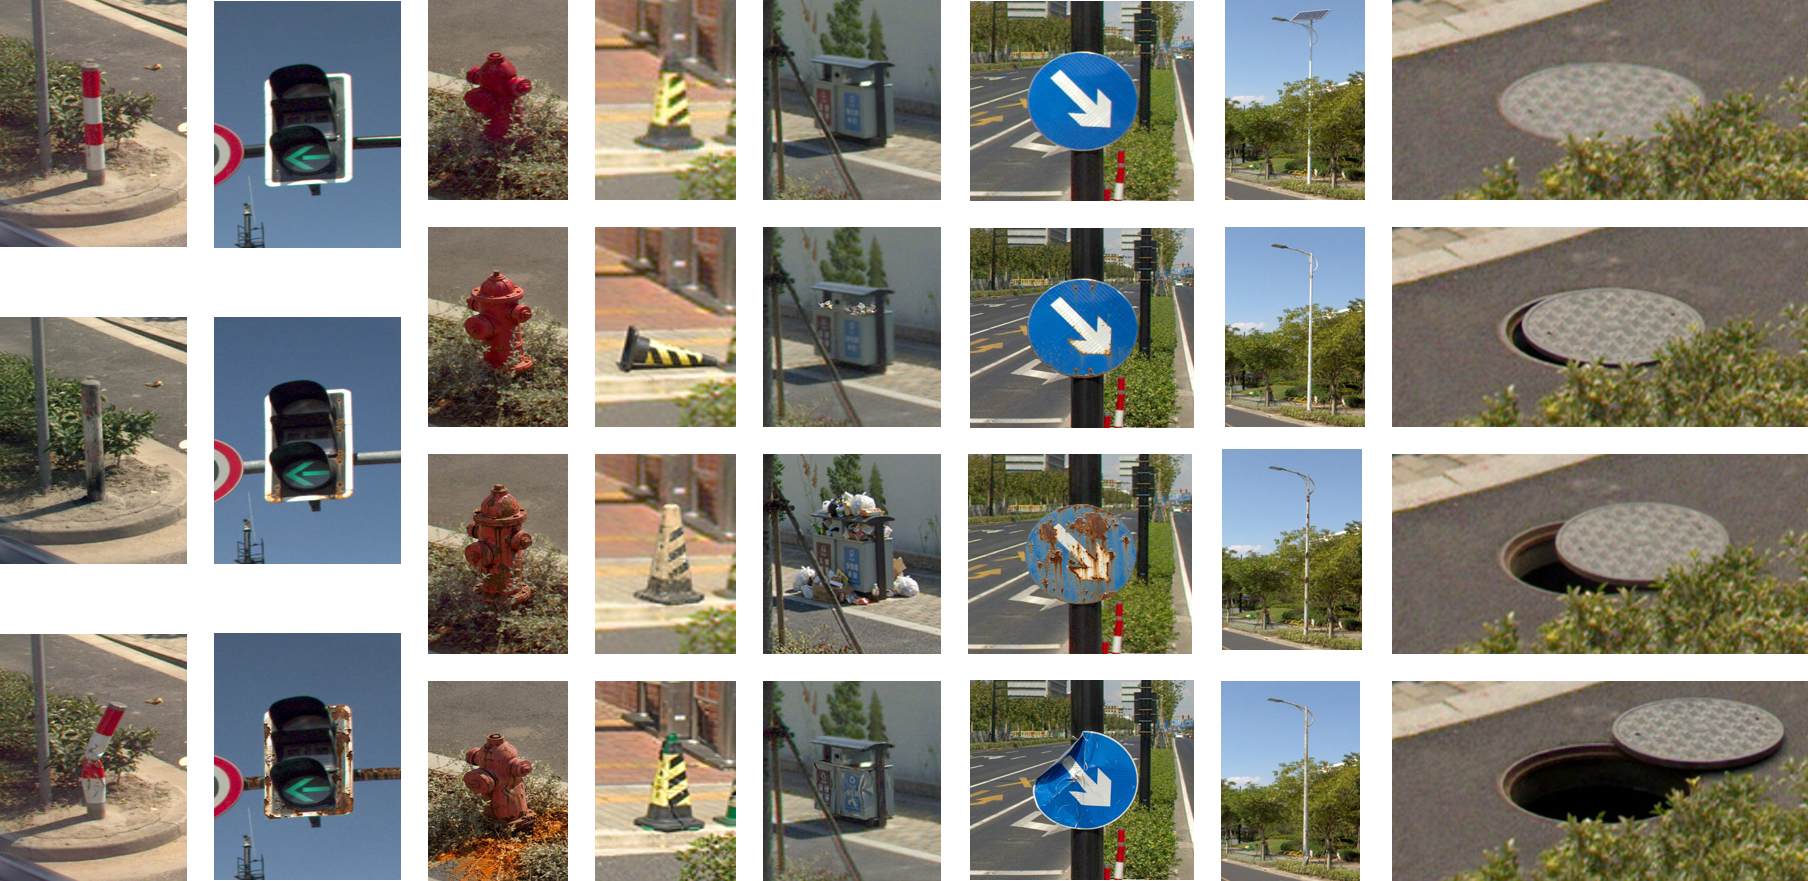
\includegraphics[width=1.0\textwidth]{logo/gemini-3.0-pro-image 生成不同异常等级样本的稳定性与阶梯一致性示例.png}
    \caption{gemini-3.0-pro-image 生成不同异常等级样本的稳定性与阶梯一致性示例}
    \label{fig:gemini_stability_levels}
\end{figure}

\subsubsection{主生成模型的批量构造方式}

在完成候选模型比较后，本文确定 gemini-3.0-pro-image 作为统一的主生成模型，并直接使用该模型批量构造异常属性样本。具体做法是：围绕交通标志牌、路灯、信号灯、井盖、垃圾桶等对象，预先设定异常类型、异常等级和局部编辑约束，再结合对应的参考图像逐类批量生成所需样本。

这种做法的重点不在于对每一条生成结果再额外进行复杂筛选，而在于通过前期模型比较与 Prompt 约束设计，先确定一个在结构保持、异常表达和背景稳定性方面都较为可靠的生成模型，然后利用统一生成方案成规模补足长尾异常属性空间。由此获得的生成样本主要服务于训练分布扩充，而后续是否真正带来识别增益，则由本章后续对照实验统一验证。

\subsection{长尾补样后的数据分布结果}

\subsubsection{训练集异常子集补充效果}

本文的核心实验动机来自训练集分布的显著差异。表~\ref{tab:tail_coverage_train} 统计了两份训练数据中若干代表性异常属性值的样本数。其中，仅真实样本训练集由 6000 张真实样本组成；长尾增强训练集则在这 6000 张真实样本基础上进一步加入 3600 条生成异常样本。为避免不同对象中语义等价但字段名不同的异常被分散统计，表中对代表性异常属性进行了统一归并：锈蚀与风化老旧统一计入“老化情况”，弯曲与结构性受损统一计入“损坏情况”。可以看到，仅真实样本训练集虽然覆盖了大量真实常规场景，但在多个关键异常字段上几乎为空白；而长尾增强训练集则通过长尾补充样本显著扩展了异常属性空间。

\begin{table}[htbp]
\centering
\caption{两种训练集在代表性异常属性值上的覆盖情况}
\label{tab:tail_coverage_train}
\setlength{\tabcolsep}{5pt}
\begin{tabular}{llcc}
\toprule
\textbf{属性} & \textbf{属性值} & \textbf{仅真实样本训练集} & \textbf{长尾增强训练集}\\
\midrule
损坏情况 & 中级锈蚀+弯曲 & 0 & 439\\
损坏情况 & 结构损坏 & 7 & 158\\
损坏情况 & 严重损坏 & 0 & 66\\
老化情况 & 初级锈蚀 & 0 & 700\\
老化情况 & 中级锈蚀 & 0 & 700\\
老化情况 & 风化/老旧 & 5 & 66\\
隐患情况 & 微微移位 & 0 & 91\\
隐患情况 & 移开一半 & 0 & 91\\
隐患情况 & 完全移开 & 0 & 91\\
垃圾是否装满 & 满至边缘 & 3 & 160\\
垃圾是否装满 & 溢出 & 0 & 159\\
\bottomrule
\end{tabular}
\end{table}

上述统计说明，长尾增强训练集并不是简单增加了样本数量，而是在保持真实数据主体结构的同时，系统性补齐了多个对巡检具有重要意义的异常属性值。这一点对于后续模型性能的解释至关重要：如果 $M_{\mathrm{aug}}$ 在统一测试集上优于 $M_{\mathrm{real}}$，则这种提升更有可能来自异常属性覆盖增强，而非单纯的数据规模放大。

\subsubsection{测试集异常挑战性分析}

统一测试集并非只包含常规真实样本，而是由 1311 张真实样本和 597 条生成异常样本共同构成，同时覆盖常规场景与异常长尾场景。表~\ref{tab:test_tail_distribution} 进一步按数据来源给出了测试集中四类关键异常子集的分布情况。可以看到，除“隐患情况”全部来自长尾增强样本外，其余三类异常子集均同时包含少量真实样本与大量增强样本。这说明统一测试集不仅能够检验模型对补充异常模式的识别能力，也保留了对真实异常样本识别表现的基本观察依据。

\begin{table}[htbp]
\centering
\caption{统一测试集中关键异常子集按数据来源的分布情况}
\label{tab:test_tail_distribution}
\setlength{\tabcolsep}{5pt}
\begin{tabular}{lccc}
\toprule
\textbf{异常子集} & \textbf{真实样本} & \textbf{长尾增强样本} & \textbf{合计}\\
\midrule
损坏情况 & 3 & 141 & 144\\
老化情况 & 4 & 251 & 255\\
隐患情况 & 0 & 43 & 43\\
垃圾桶是否装满 & 2 & 50 & 52\\
\bottomrule
\end{tabular}
\end{table}

这表明，本文实验并非在缺乏异常样本的测试场景中考察模型，而是在包含明确异常标签、且区分了真实来源与增强来源的测试集上验证生成数据的有效性。因此，后续若观察到 $M_{\mathrm{aug}}$ 在异常属性上的稳定提升，将能够更直接地支撑“生成长尾数据具有实际价值”这一论断。

\subsection{知识引导长尾增强效果分析}

\subsubsection{领域知识引导促进作用的核心对照结果}

围绕统一测试集上的核心对照实验，本文重点比较了仅真实样本训练模型 $M_{\mathrm{real}}$ 与长尾增强训练模型 $M_{\mathrm{aug}}$ 的识别表现。为使异常子集划分更符合交通养护语义，本文将原始异常值进一步归并为四类：\textbf{损坏情况}（结构损坏、严重损坏、弯曲等）、\textbf{老化情况}（初级/中级锈蚀、风化老旧等）、\textbf{隐患情况}（井盖移位等）以及\textbf{垃圾桶是否装满}（满至边缘、溢出）。在此定义下，$M_{\mathrm{aug}}$ 在样本级严格准确率、属性级准确率以及异常属性准确率三个层面均显著优于 $M_{\mathrm{real}}$：其 $\mathrm{Acc}_{\mathrm{inst}}$、$\mathrm{Acc}_{\mathrm{attr}}$ 与 $\mathrm{Acc}_{\mathrm{abn}}$ 分别达到 88.78\%、96.12\% 和 93.72\%，相比 $M_{\mathrm{real}}$ 的 57.97\%、84.52\% 和 1.01\% 分别提升了 30.82、11.60 和 92.71 个百分点。这说明长尾增强训练不仅提升了整体属性识别效果，也显著改善了模型对低频风险状态的判别能力。

进一步从正常属性保持能力来看，$M_{\mathrm{aug}}$ 并未因引入生成样本而在常规属性上出现明显退化。相反，其 $\mathrm{Acc}_{\mathrm{norm}}$ 从 96.64\% 进一步提升至 99.81\%，同时正常--异常性能差距 $\mathrm{Gap}$ 由 95.63\% 大幅缩小至 6.08\%。这说明领域知识引导生成带来的价值并不只是增加数据量，而是在补齐长尾异常属性后，使模型能够在保持正常样本识别能力的同时，更稳定地区分“正常磨损”“轻微异常”和“明显异常”之间的边界。

表~\ref{tab:recognition_main_results} 给出了统一测试集上的总体识别结果对比。其中，$\mathrm{Acc}_{\mathrm{abn}}$ 仅在上述四类关键异常子集上统计。可以看到，在两组经过任务化训练的模型中，长尾增强训练模型 $M_{\mathrm{aug}}$ 在五项总体指标上均显著优于仅真实样本训练的 $M_{\mathrm{real}}$。若与零样本商用多模态模型相比，$M_{\mathrm{aug}}$ 同样取得了最优的总体表现；而 $M_{\mathrm{real}}$ 虽然在 $\mathrm{Acc}_{\mathrm{inst}}$、$\mathrm{Acc}_{\mathrm{attr}}$ 和 $\mathrm{Acc}_{\mathrm{norm}}$ 上仍高于三种商用模型，但其 $\mathrm{Acc}_{\mathrm{abn}}$ 仅为 1.01\%，明显低于商用模型的 45.95\%--54.66\%，说明仅依赖真实训练样本时，模型对关键长尾异常几乎不具备有效识别能力。

\begin{table}[htbp]
\centering
\caption{统一测试集上不同识别模型的总体性能对比}
\label{tab:recognition_main_results}
\begin{tabular}{lccccc}
\toprule
\textbf{模型} & $\mathbf{Acc_{inst}}$ & $\mathbf{Acc_{attr}}$ & $\mathbf{Acc_{abn}}$ & $\mathbf{Acc_{norm}}$ & \textbf{Gap}\\
\midrule
$M_{\mathrm{real}}$ & 57.97\% & 84.52\% & 1.01\% & 96.64\% & 95.63\%\\
$M_{\mathrm{aug}}$ & 88.78\% & 96.12\% & 93.72\% & 99.81\% & 6.08\%\\
Gemini-2.5-Flash & 31.24\% & 45.97\% & 50.75\% & 40.48\% & -10.27\%\\
gpt-5.3-chat-latest & 33.02\% & 69.70\% & 45.95\% & 90.38\% & 44.43\%\\
Doubao-Seed-2.0-Pro & 33.12\% & 53.17\% & 54.66\% & 55.58\% & 0.92\%\\
\bottomrule
\end{tabular}
\end{table}

除总体指标外，关键异常子类的识别结果同样需要单独呈现。为避免与原始字段名混淆，表~\ref{tab:recognition_key_attr_results} 按照语义定义的四类异常子集统计准确率：其中“损坏情况”对应结构损坏、严重损坏和弯曲类状态，“老化情况”对应锈蚀与风化老旧状态。可以看到，$M_{\mathrm{aug}}$ 在这四个关键异常子类上均取得了最优结果，而 $M_{\mathrm{real}}$ 在“损坏情况”“老化情况”和“隐患情况”三个核心长尾子类上的准确率均为 0。

\begin{table}[htbp]
\centering
\caption{不同识别模型在关键异常子集上的准确率对比}
\label{tab:recognition_key_attr_results}
\begin{tabular}{lcccc}
\toprule
\textbf{模型} & \textbf{损坏情况} & \textbf{老化情况} & \textbf{隐患情况} & \textbf{垃圾桶是否装满}\\
\midrule
$M_{\mathrm{real}}$ & 0.00\% & 0.00\% & 0.00\% & 9.62\%\\
$M_{\mathrm{aug}}$ & 93.75\% & 94.51\% & 81.40\% & 100.00\%\\
Gemini-2.5-Flash & 36.67\% & 61.96\% & 74.42\% & 46.15\%\\
gpt-5.3-chat-latest & 25.69\% & 48.63\% & 69.77\% & 69.23\%\\
Doubao-Seed-2.0-Pro & 32.64\% & 58.43\% & 76.74\% & 78.85\%\\
\bottomrule
\end{tabular}
\end{table}

此外，为解释生成样本究竟带来了“记忆生成样本”还是“提升异常判别边界”两种不同效应，本文进一步按样本来源对子集结果进行切片。表~\ref{tab:recognition_source_split_results} 给出了真实来源子集与生成增强来源子集上的分组评测结果。可以看到，$M_{\mathrm{aug}}$ 在真实来源子集上并未退化，在增强来源子集上则表现出显著优势。

\begin{table}[htbp]
\centering
\caption{不同识别模型按样本来源切片的结果对比}
\label{tab:recognition_source_split_results}
\resizebox{\textwidth}{!}{
\begin{tabular}{lcccccc}
\toprule
\textbf{模型} & \textbf{真实来源} $Acc_{inst}$ & \textbf{真实来源} $Acc_{attr}$ & \textbf{真实来源} $Acc_{abn}$ & \textbf{增强来源} $Acc_{inst}$ & \textbf{增强来源} $Acc_{attr}$ & \textbf{增强来源} $Acc_{abn}$\\
\midrule
$M_{\mathrm{real}}$ & 84.36\% & 93.82\% & 0.00\% & 0.00\% & 65.00\% & 1.02\%\\
$M_{\mathrm{aug}}$ & 86.73\% & 95.16\% & 0.00\% & 93.30\% & 98.14\% & 94.49\%\\
\bottomrule
\end{tabular}
}
\end{table}

\subsubsection{商用多模态大模型基线对照}

为进一步说明长尾增强训练的必要性，本文还在同一测试集上统计了三种商用多模态大模型零样本基线结果，分别为 Gemini-2.5-Flash、gpt-5.3-chat-latest 和 Doubao-Seed-2.0-Pro。其总体指标已汇总于表~\ref{tab:recognition_main_results}。在采用语义等价归并与字段别名映射后的统一评测口径下，Gemini-2.5-Flash 的 $\mathrm{Acc}_{\mathrm{inst}}$ 和 $\mathrm{Acc}_{\mathrm{attr}}$ 分别为 31.24\% 和 45.97\%，gpt-5.3-chat-latest 分别为 33.02\% 和 69.70\%，Doubao-Seed-2.0-Pro 分别为 33.12\% 和 53.17\%。在异常子集上，三者的 $\mathrm{Acc}_{\mathrm{abn}}$ 分别为 50.75\%、45.95\% 和 54.66\%；对应的 $\mathrm{Acc}_{\mathrm{norm}}$ 分别为 40.48\%、90.38\% 和 55.58\%。其中，gpt-5.3-chat-latest 在常规属性识别上最强，Doubao-Seed-2.0-Pro 在商用模型中取得了最高的样本级准确率和异常属性准确率，而 Gemini-2.5-Flash 的正常属性准确率甚至低于其异常属性准确率，因而呈现负的 $\mathrm{Gap}$。总体上，三种商用模型在结构化多属性联合识别上的稳定性仍明显弱于经过长尾增强训练的 $M_{\mathrm{aug}}$。

进一步考察关键异常子集，可见商用模型对任务相关长尾属性的识别稳定性仍然不足。Gemini-2.5-Flash 在“损坏情况”“老化情况”“隐患情况”和“垃圾桶是否装满”上的准确率分别为 36.67\%、61.96\%、74.42\% 和 46.15\%；gpt-5.3-chat-latest 对应指标分别为 25.69\%、48.63\%、69.77\% 和 69.23\%；Doubao-Seed-2.0-Pro 对应指标分别为 32.64\%、58.43\%、76.74\% 和 78.85\%。可以看到，在三种商用模型中，Gemini-2.5-Flash 在“损坏情况”和“老化情况”两类异常上相对更强，Doubao-Seed-2.0-Pro 在“隐患情况”和“垃圾桶是否装满”上表现最佳，而 gpt-5.3-chat-latest 虽在总体 $\mathrm{Acc}_{\mathrm{attr}}$ 上最高，但在四类关键异常子集上均未取得最优结果。相比之下，$M_{\mathrm{aug}}$ 在四个关键异常子集上的准确率分别达到 93.75\%、94.51\%、81.40\% 和 100.00\%，均显著高于商用模型，说明长尾增强训练对细粒度异常属性的识别促进作用是稳定且全面的。

综合来看，本文的核心结论并非“商用大模型完全无法识别异常”，而是“若没有面向任务的长尾异常数据与监督微调，再强的通用模型也难以在结构化、细粒度、工程约束强的交通资产识别任务中获得稳定结果”。这也从侧面说明了构建知识引导长尾补充数据集的必要性。

\subsection{结果讨论与局限性分析}

\subsubsection{整体增益特征}

从总体结果看，知识引导长尾增强带来的收益不仅体现在单一字段准确率提升上，更体现在结构化多属性联合识别能力的整体改善上。样本级严格准确率 $\mathrm{Acc}_{\mathrm{inst}}$ 由 57.97\% 提升至 88.78\%，属性级准确率 $\mathrm{Acc}_{\mathrm{attr}}$ 由 84.52\% 提升至 96.12\%，说明增强后的训练分布同时改善了单字段判别质量与多字段联合输出一致性。考虑到交通资产属性识别属于典型的结构化预测任务，任一关键字段预测错误都可能导致样本级结果失效，因此样本级指标的大幅提升表明，知识引导长尾增强对整体判别边界具有实质性促进作用，而非仅对个别属性产生局部修正。

\subsubsection{关键异常属性增益}

相较于总体平均指标，本文更关注关键异常子集上的识别增益。由表~\ref{tab:recognition_main_results} 和表~\ref{tab:recognition_key_attr_results} 可见，$M_{\mathrm{aug}}$ 的异常属性准确率 $\mathrm{Acc}_{\mathrm{abn}}$ 由 1.01\% 提升至 93.72\%，正常--异常性能差距 $\mathrm{Gap}$ 由 95.63\% 缩小至 6.08\%。这一结果表明，知识引导长尾增强并未进一步强化模型对高频正常类的偏置，而是显著提升了其对低频异常模式的辨识能力。进一步结合四类关键异常子集可知，增益最显著的恰为原始真实训练集中最为稀缺的异常属性，说明本文方法有效实现了面向异常缺口的定向补样。

\subsubsection{样本来源切片结果解释}

统一测试集同时包含真实来源样本与生成增强来源样本，因此按样本来源进行切片分析，有助于辨析模型增益的来源。由表~\ref{tab:recognition_source_split_results} 可见，$M_{\mathrm{aug}}$ 在真实来源子集上的 $\mathrm{Acc}_{\mathrm{inst}}$ 和 $\mathrm{Acc}_{\mathrm{attr}}$ 分别达到 86.73\% 和 95.16\%，均不低于 $M_{\mathrm{real}}$；在增强来源子集上，其 $\mathrm{Acc}_{\mathrm{inst}}$、$\mathrm{Acc}_{\mathrm{attr}}$ 和 $\mathrm{Acc}_{\mathrm{abn}}$ 则分别达到 93.30\%、98.14\% 和 94.49\%，表现出明显优势。该结果说明，长尾增强并未破坏模型对真实样本分布的适应能力，同时显著提升了模型对补充异常模式的识别性能。因而，本文方法带来的收益更可理解为异常属性空间得到有效补齐后形成的判别边界改善，而非对生成样本的简单记忆。

\subsubsection{工程意义与局限性}

从工程应用角度看，本文方法提供了一条面向交通资产异常属性识别的可扩展数据构建路径。与完全依赖真实异常采集相比，知识引导生成能够以较低成本补充锈蚀、结构损坏、井盖移位和垃圾满溢等关键低频风险状态，从而提高模型在实际巡检场景中的异常识别能力与结构化记录质量。

同时，本文方法仍存在一定局限。首先，尽管生成样本受到领域知识约束，其分布与真实异常图像之间仍可能存在差异；其次，不同异常类型的生成稳定性并不一致，结构性破坏通常较纹理性异常更难准确建模；再次，当前统一测试集虽然同时包含真实来源样本与增强来源样本，但对极端道路环境和更复杂异常组合的覆盖仍有限。后续可通过补充真实异常采集、加强人工复核以及细化生成约束等方式，进一步提高增强数据的真实性与工程可用性。

\section{本章小结}

本章围绕交通资产属性识别增强问题，系统阐述了领域知识引导长尾数据生成的方法设计及其实验验证过程。方法层面，本文从任务定义、知识约束表达、异常样本构建、生成模型比较与批量构造以及属性识别训练范式五个方面，构建了面向交通资产异常属性补样的完整技术路线；验证层面，本文以从 WHU-Infra3D 数据集中筛选得到的 7311 张真实局部样本为基础，并结合 4197 条领域知识引导生成的异常属性样本，构造了仅真实数据训练模型 $M_{\mathrm{real}}$ 与长尾增强训练模型 $M_{\mathrm{aug}}$ 两组核心对照，同时补充引入商用多模态大模型零样本基线进行比较。

实验结果表明，领域知识引导生成的长尾补充数据显著扩展了训练集中的关键异常属性覆盖范围，使识别模型在整体属性识别、关键异常字段识别以及正常--异常性能平衡方面均获得明显改善。与此同时，商用大模型基线结果进一步说明：若缺少任务相关的长尾异常数据支持，即使具备较强通用视觉理解能力的商业模型，在本任务中仍难以获得稳定可靠的结构化属性识别结果。总体而言，本章从真实数据筛选、长尾补样构建、模型对照与结果分析四个层面验证了领域知识引导长尾数据生成对交通资产属性识别任务的实际价值。
